\documentclass{article}
\usepackage[T1]{fontenc}
\usepackage{lmodern}
\usepackage{graphicx}
\usepackage{amsmath,amssymb}
\usepackage[a4paper,margin=2cm]{geometry}
\usepackage[absolute,overlay]{textpos}
\setlength{\TPHorizModule}{1mm}
\setlength{\TPVertModule}{1mm}
\usepackage[indonesian]{babel}
\usepackage{hyperref}
\setlength{\emergencystretch}{2em}
% unit: Halaman 75

\begin{document}

% === Halaman 75 (llm) ===

\vspace{154.44mm}

\begin{verbatim}
# Sisipkan bit-bit pesan pada LSB setiap byte
index = 0
for p in range(total_pixel):
    for q in range(3):
        if index < panjang_bit_pesan:
            larik_pixel[p][q] = (larik_pixel[p][q] & 254) | int(pesan_biner[index])
            # 254 = 11111110 dalam biner
            index = index + 1

larik_pixel = larik_pixel.reshape(tinggi, lebar, n)
stego_image = Image.fromarray(larik_pixel.astype('uint8'), citra.mode)
stego_image.save(stego)
print("Penyisipan pesan ke dalam citra berhasil")
\end{verbatim}

% deskripsi: Cuplikan kode pemrograman Python untuk implementasi teknik steganografi Least Significant Bit (LSB).
% bbox normalisasi: [0.0500, 0.1000, 0.9500, 0.6200]
\begin{textblock*}{189.00mm}(10.50mm,29.70mm)
\noindent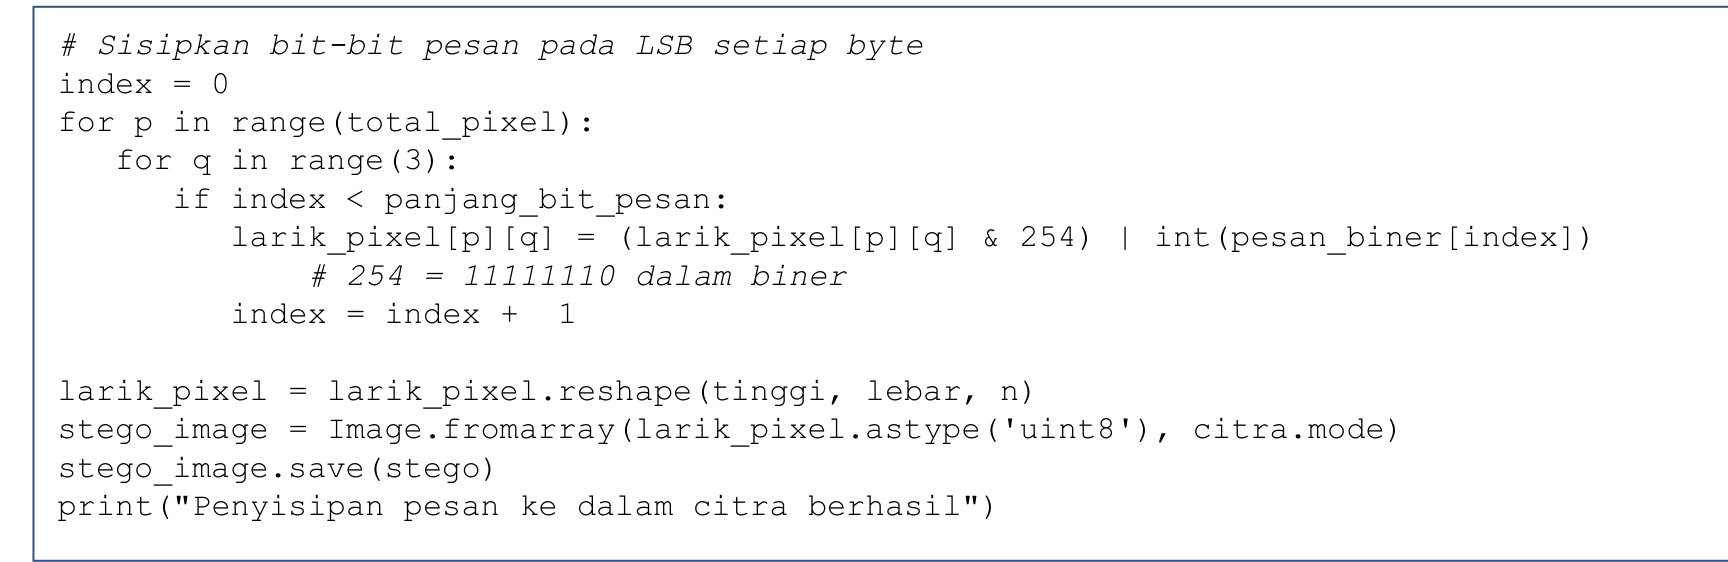
\includegraphics[width=189.00mm,height=154.44mm]{../../images/llm/page_075_img_01.png}%
\end{textblock*}

\end{document}
